% =====================================================================
%  Raman-AI : Defense Presentation -- 20-MINUTE COMPACT VERSION
%  Mathematical-density first; data-scarcity is the only limitation.
%  Compile:  latexmk -pdf presentation_short.tex
% =====================================================================
\documentclass[10pt,aspectratio=169]{beamer}

\usetheme[progressbar=frametitle, numbering=fraction, block=fill]{metropolis}
\setbeamertemplate{frame numbering}[fraction]
\setbeamercolor{progress bar}{fg=Maroon}
\setbeamercolor{alerted text}{fg=Maroon}

\usepackage[utf8]{inputenc}
\usepackage[T1]{fontenc}
\usepackage{lmodern}
\usepackage{microtype}
\usepackage{amsmath, amssymb, amsthm, mathtools, bm}
\usepackage{booktabs}
\usepackage{array}
\usepackage{siunitx}
\usepackage{xcolor}
\usepackage{tikz}
\usetikzlibrary{positioning, arrows.meta, shapes.geometric, fit, calc,
                shadows.blur}
\usepackage[ruled,vlined,linesnumbered]{algorithm2e}
\usepackage{pifont}
\usepackage[backend=biber,style=numeric,sorting=none,
            maxbibnames=4, doi=false, isbn=false, url=false]{biblatex}
\addbibresource{references.bib}

\definecolor{ink}{HTML}{1A1A1A}
\definecolor{accent}{HTML}{7C5C3E}
\definecolor{accentTwo}{HTML}{4D6880}
\definecolor{good}{HTML}{2E5938}
\definecolor{bad}{HTML}{6E2E2E}

\newcommand{\good}[1]{\textcolor{good}{\textbf{#1}}}
\newcommand{\bad}[1]{\textcolor{bad}{\textbf{#1}}}
\newcommand{\code}[1]{\texttt{\small #1}}
\newcommand{\cmone}{\si{\per\centi\meter}}

% Math shortcuts
\newcommand{\R}{\mathbb{R}}
\newcommand{\E}{\mathbb{E}}
\newcommand{\norm}[1]{\left\lVert #1 \right\rVert}
\newcommand{\inner}[2]{\left\langle #1,\, #2 \right\rangle}
\DeclareMathOperator*{\argmin}{arg\,min}
\DeclareMathOperator*{\argmax}{arg\,max}
\DeclareMathOperator{\interp}{interp}
\DeclareMathOperator{\SG}{SG}
\DeclareMathOperator{\ALS}{ALS}
\DeclareMathOperator{\CR}{CR}

\title[Raman-AI]{\textbf{A Hybrid Spectral-Matching and Deep-Learning System\\[0.18em]
        for Real-Time Mineral Identification\\[0.18em] from Raman Spectra}}
\subtitle{Final Project Defense \,\textbar\, 20-minute talk}
\author[Rahul]{\textbf{Rahul \textit{[Surname]}}\\[0.3em]
        \small Under the supervision of \textit{[Advisor Name]}}
\institute{Department of \textit{[Discipline]} \,\textbar\, \textit{[Institution Name]}}
\date{\today}

\begin{document}

% ----------------------------------------------------------------- 1
\maketitle

% ----------------------------------------------------------------- 2
\begin{frame}{Problem statement}
\textbf{Inputs.} Unknown Raman measurement
$\mathbf{q}_{\text{raw}} = \{(\nu_i, I_i)\}_{i=1}^{N}$;
reference library $\mathcal{R} = \{\mathbf{r}_m\}_{m=1}^{M}$
on a canonical grid $\bm{\nu}_{*} \in \R^{P}$,
$P{=}1951$, $\Delta\nu{=}\SI{2}{\per\centi\meter}$, range $[100, 4000]\,\cmone$.
\medskip

\textbf{Outputs.}
\begin{enumerate}
  \item Ranked identifications $\bigl((m_{(k)}, c_{(k)})\bigr)_{k=1}^{K}$,
        confidences $c_{(k)} \in [0,1]$.
  \item Mixture weights
        $\mathbf{x}^{\star} \in \R_{\geq 0}^{|\mathcal{C}|}$ minimising
        $\norm{A_{\mathcal{C}}^{\!\top}\mathbf{x} - \tilde{\mathbf{q}}}_{2}$
        over a candidate index set $\mathcal{C} \subseteq [M]$.
\end{enumerate}
\medskip

\textbf{Constraint.} End-to-end latency
$\tau \leq \SI{1}{\second}$ on a single laptop GPU.
\medskip

\textbf{Two design questions.}
(i) When does a learned classifier outperform classical spectral matching?
(ii) How are the two reconciled at inference?
\end{frame}

% ----------------------------------------------------------------- 3
\begin{frame}{System architecture}
\begin{center}
\resizebox{0.95\textwidth}{!}{%
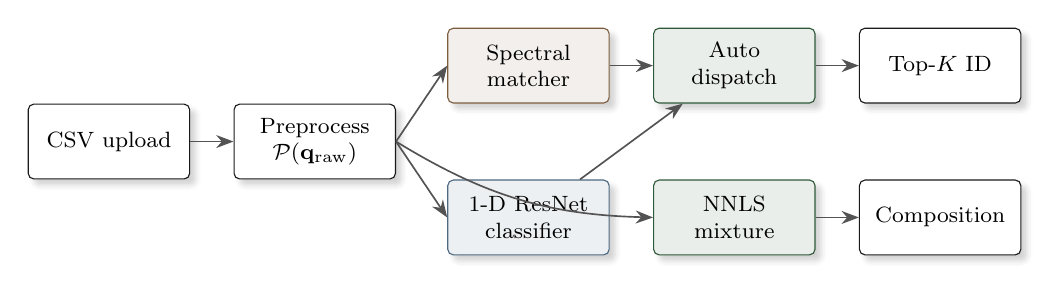
\begin{tikzpicture}[
    node distance=0.45cm and 0.55cm,
    box/.style={draw=ink, rounded corners=2pt, fill=white, font=\footnotesize,
                align=center, minimum height=0.95cm, minimum width=2.05cm,
                blur shadow={shadow blur radius=2pt, shadow opacity=18}},
    ml/.style ={box, draw=accentTwo, fill=accentTwo!10},
    cl/.style ={box, draw=accent, fill=accent!10},
    ag/.style ={box, draw=good, fill=good!10},
    arr/.style={-{Stealth[length=2.2mm]}, semithick, draw=ink!75}]

  \node[box] (csv)   {CSV upload};
  \node[box, right=of csv]                      (pre)  {Preprocess\\$\mathcal{P}(\mathbf{q}_{\text{raw}})$};
  \node[cl, above right=0.0 and 0.65 of pre]    (mat)  {Spectral\\matcher};
  \node[ml, below right=0.0 and 0.65 of pre]    (cnn)  {1-D ResNet\\classifier};
  \node[ag, right=of mat]                       (disp) {Auto\\dispatch};
  \node[ag, right=of cnn]                       (mix)  {NNLS\\mixture};
  \node[box, right=0.55 of disp] (idr) {Top-$K$ ID};
  \node[box, right=0.55 of mix]  (mxr) {Composition};

  \draw[arr] (csv) -- (pre);
  \draw[arr] (pre.east) -- (mat.west);
  \draw[arr] (pre.east) -- (cnn.west);
  \draw[arr] (mat) -- (disp);
  \draw[arr] (cnn) -- (disp);
  \draw[arr] (pre.east) to[bend right=15] (mix.west);
  \draw[arr] (disp) -- (idr);
  \draw[arr] (mix)  -- (mxr);
\end{tikzpicture}}
\end{center}
\smallskip
\footnotesize
\textbf{Two identifiers, one dispatcher.} Spectral matching always runs as a
deterministic safety net; the learned classifier enters the comparison only
above a calibrated confidence threshold. NNLS decomposes the
preprocessed spectrum independently of the identifier.
\end{frame}

% ----------------------------------------------------------------- 4
\begin{frame}{Preprocessing pipeline $\mathcal{P}: \mathbf{q}_{\text{raw}} \mapsto \tilde{\mathbf{q}}$}
\[
  \mathcal{P} \;=\;
    \underbrace{\ell_{2}}_{\text{normalise}}\;\circ\;
    \underbrace{(\,\cdot\,)_{+}}_{\text{clip}}\;\circ\;
    \underbrace{(I - \ALS_{\lambda, p})}_{\text{baseline removal}}\;\circ\;
    \SG_{w=5,\, p=3}\;\circ\;\CR_{\rho=5}\;\circ\;
    \underbrace{\interp_{\bm{\nu}_{*}}}_{\text{canonical grid}}.
\]
\smallskip

\textbf{ALS baseline} \cite{eilers2005baseline}. Find $\mathbf{z}$ minimising
\[
  \mathcal{F}(\mathbf{z}) \;=\;
   \sum_{i} w_{i}\,(y_{i} - z_{i})^{2}
   \;+\; \lambda\,\norm{D_{2}\mathbf{z}}_{2}^{2},
   \qquad
   w_{i} \;=\;
   \begin{cases} p,         & y_{i} > z_{i},\\
                 1 - p,     & y_{i} \leq z_{i},
   \end{cases}
\]
solved by iterating
$(W + \lambda D_{2}^{\!\top} D_{2})\,\mathbf{z} = W\mathbf{y}$
with $\lambda = 10^{5}$, $p = 0.01$.
\smallskip

\begin{block}{Order matters}
$\interp$ \emph{first} guarantees a constant physical Savitzky–Golay window
$w_{\text{phys}} = w \cdot \Delta\nu = 10\,\cmone$ across all inputs.
On the raw grid $w_{\text{phys}}$ would scale with the spectrometer step
$\delta\nu_{\text{raw}}$, producing a $44\,\cmone$ window for a
\SI{4}{\per\centi\meter} CSV --- wide enough to merge Raman doublets.
\end{block}
\end{frame}

% ----------------------------------------------------------------- 5
\begin{frame}{Reference database $A \in \R^{(M_{s} + M_{r}) \times P}$}
For every mineral with a curated synthetic profile we keep
\emph{both} the synthetic row $\mathbf{r}_{m}^{\,s}$
and the RRUFF-averaged row $\mathbf{r}_{m}^{\,r}$:
\[
  A \;=\;
  \begin{bmatrix}
    \mathbf{r}_{1}^{\,s} & \cdots & \mathbf{r}_{M_{s}}^{\,s} &
    \mathbf{r}_{1}^{\,r} & \cdots & \mathbf{r}_{M_{r}}^{\,r}
  \end{bmatrix}^{\!\top},
  \qquad
  M_{s}{=}25,\; M_{r}{=}2477,\; P{=}1951.
\]
\smallskip

\textbf{Cardinality.}
\;$\dim A = 2502 \times 1951$;
\;unique display names $|\mathrm{names}(A)| = 2481$
(of which $21$ minerals contribute two rows).
\smallskip

\textbf{Result-time deduplication.} For each mineral $m$,
\[
  \hat{\imath}(m) \;=\; \argmax_{i\,:\,\text{name}(i)\,=\,m}\; s\!\left(\tilde{\mathbf{q}},\,\mathbf{r}_{i}\right).
\]
\medskip

\begin{block}{Why two sources?}
Synthetic rows are the canonical anchor for low-noise queries
(perfect Lorentzian template); RRUFF averages carry instrumental
bandshape needed for noisy real-world queries. Keeping only one of
the two collapsed identification accuracy by $\sim 20$ percentage points
on whichever regime was unrepresented.
\end{block}
\end{frame}

% ----------------------------------------------------------------- 6
\begin{frame}{Combined-metric spectral matcher}
For preprocessed query $\tilde{\mathbf{q}}$ and reference $\mathbf{r}_{m}$,
\[
  \boxed{\;
  s\!\left(\tilde{\mathbf{q}},\,\mathbf{r}_{m}\right)
  \;=\;
  \tfrac{1}{2}\,\inner{\hat{\mathbf{q}}}{\hat{\mathbf{r}}_{m}}
  \;+\;
  \tfrac{1}{2}\,\inner{\widehat{D^{2}\!\tilde{\mathbf{q}}}}{\widehat{D^{2}\!\mathbf{r}_{m}}}
  \;}
\]
where $D^{2}$ is the SG second-derivative operator and
$\hat{\mathbf{v}} \,=\, (\mathbf{v} - \bar{\mathbf{v}}\bm{1})\,/\,\norm{\mathbf{v}-\bar{\mathbf{v}}\bm{1}}$
is the mean-centred unit-norm transform.
\medskip

\textbf{Two failure modes that motivate the blend:}
\begin{itemize}\setlength\itemsep{0.2em}
  \item Cosine alone --- sensitive to broad bandshape; over-rewards a RRUFF
        average that drifts in the same direction as $\tilde{\mathbf{q}}$.
  \item $D^{2}$-Pearson alone --- emphasises peak position; ties unrelated
        minerals sharing a peak within $\pm \delta\nu$.
\end{itemize}
\medskip

\textbf{Equal-weight blend} lets each metric \alert{veto} the other.
Weights selected by 1-D grid search on a held-out RRUFF panel; objective
plateaued in $[0.4, 0.6]$.
\end{frame}

% ----------------------------------------------------------------- 7
\begin{frame}{1-D residual classifier $f_{\theta}: \R^{P} \to \Delta^{C}$}
\centering
\begin{tabular}{@{}llr@{}}
\toprule
\textbf{Stage} & \textbf{Operation} & \textbf{Output}\\
\midrule
Stem-1 & $\mathrm{Conv}_{k=25,s=2}$ + BN + GELU & $(B,32,488)$\\
Stem-2 & $\mathrm{Conv}_{k=15,s=2}$ + BN + GELU & $(B,32,244)$\\
Stage-1 & $3 \times \mathrm{ResBlock}(32,k{=}7)$ & $(B,32,244)$\\
Down   & $\mathrm{Conv}_{k=5,s=2}$ + BN + GELU & $(B,64,122)$\\
Stage-2 & $3 \times \mathrm{ResBlock}(64,k{=}5)$ & $(B,64,122)$\\
Pool   & AdaptiveAvgPool1D & $(B,64)$\\
Head   & $\mathrm{FC}_{64\to 512} \to \mathrm{GELU} \to \mathrm{FC}_{512\to C}$ & $(B,C)$\\
\midrule
\multicolumn{2}{l}{\textbf{Parameters}} & $\mathbf{6.6 \times 10^{5}}$ \\
\bottomrule
\end{tabular}
\smallskip

\raggedright
\textbf{Training objective.}
$\mathcal{L} = \mathrm{CE}_{\varepsilon=0.1}(f_{\theta}(\tilde{\mathbf{x}}_{\mathrm{aug}}), y)
   + \mathrm{Mixup}(\alpha{=}0.4)$.
Optimiser AdamW \cite{loshchilov2019adamw} with OneCycleLR
\cite{smith2019onecycle}, peak $\eta = 10^{-3}$, weight decay $10^{-4}$.
Class space $C = 851$ after the filter $\bigl|\,\mathbf{r}_m^{r}\,\bigr| \geq 2$.
Augmentation expands each spectrum by $V = 25$ variants (noise, gain jitter,
$\pm 10\,\cmone$ shift, residual baseline, broadening, dropout).
\end{frame}

% ----------------------------------------------------------------- 8
\begin{frame}{Candidate-restricted NNLS mixture decomposition}
Solve
\[
  \mathbf{x}^{\star}
  \;=\;
  \argmin_{\mathbf{x} \,\geq\, \mathbf{0}}\;
   \norm{A_{\mathcal{C}}^{\!\top}\,\mathbf{x} \;-\; \tilde{\mathbf{q}}}_{2},
\]
with the candidate set
\[
  \mathcal{C} \;=\;
   \mathcal{C}_{\!s}
   \;\cup\;
   \Bigl\{\, m \in \mathcal{C}_{\!r}
          \;:\;
          s(\tilde{\mathbf{q}},\,\mathbf{r}_{m})
          \;>\; \max_{m' \in \mathcal{C}_{\!s}}
                s(\tilde{\mathbf{q}},\,\mathbf{r}_{m'}) \,\Bigr\}.
\]
\smallskip

\textbf{Why restrict.}
With the full library we have $|\mathcal{R}| = 2481$ unknowns vs.\ $P = 1951$
equations: \alert{underdetermined}. NNLS finds a sparse non-negative
explanation that frequently spreads credit across spectral aliases of the
dominant phase --- pure Calcite returned $0\%$ Calcite in early experiments.
Restricting $\mathcal{C}$ to the synthetic anchor plus only those RRUFF rows
that \emph{strictly exceed} the best synthetic similarity makes the system
\emph{over}-determined and the decomposition physically interpretable.
\end{frame}

% ----------------------------------------------------------------- 9
\begin{frame}{Confidence-aware dispatcher}
\begin{algorithm}[H]
\footnotesize
\DontPrintSemicolon
\KwIn{preprocessed query $\tilde{\mathbf{q}}$;
      threshold $\tau_{\min} = 0.55$}
\KwOut{ranked top-$K$ list $\mathbf{m}$, dispatch tag $\delta$}
$\mathcal{Y} \gets \emptyset$\;
$\mathbf{m}_{s} \gets \mathrm{SpectralMatch}(\tilde{\mathbf{q}})$;\quad
   $\mathcal{Y} \gets \mathcal{Y} \cup \bigl\{\,(\mathbf{m}_{s}[1].c,\,\text{matching},\,\mathbf{m}_{s})\,\bigr\}$\;
\If{CNN available}{
  $\mathbf{m}_{n} \gets f_{\theta}(\tilde{\mathbf{q}})$\;
  \lIf{$\mathbf{m}_{n}[1].c \,\geq\, \tau_{\min}$}{
       $\mathcal{Y} \gets \mathcal{Y} \cup \{(\mathbf{m}_{n}[1].c, \text{cnn}, \mathbf{m}_{n})\}$
  }
}
\If{RF available}{
  $\mathbf{m}_{r} \gets g_{\phi}(\tilde{\mathbf{q}})$\;
  \lIf{$\mathbf{m}_{r}[1].c \,\geq\, \tau_{\min}$}{
       $\mathcal{Y} \gets \mathcal{Y} \cup \{(\mathbf{m}_{r}[1].c, \text{rf}, \mathbf{m}_{r})\}$
  }
}
\Return{$\argmax_{(c, \delta, \mathbf{m})\,\in\,\mathcal{Y}}\, c$}\;
\caption{\textsc{AutoIdentify}: dispatches to the most confident identifier.}
\end{algorithm}
\smallskip
The threshold $\tau_{\min}$ is a calibration constant: in-distribution
top-1 softmax outputs cluster above $0.7$; pre-mitigation
out-of-distribution outputs lie in $[0.30,\,0.55]$.
A learned model below the threshold is \emph{ignored} and the matcher's
deterministic verdict is returned.
\end{frame}

% ----------------------------------------------------------------- 10
\begin{frame}{Results}
\textbf{Synthetic demo set.} Six CSV spectra synthesised from published peak
tables, low Gaussian noise ($\sigma = 3\!\times\!10^{-3}\,I_{\max}$).
\smallskip

\centering\small
\begin{tabular}{@{}lcrl@{}}
\toprule
Sample & Top-1 & $c_{(1)}$ & Mixture decomposition\\
\midrule
\code{quartz.csv}            & Quartz   & $99.8\%$ & Quartz $100\%$\\
\code{calcite.csv}           & Calcite  & $99.8\%$ & Calcite $100\%$\\
\code{pyrite.csv}            & Pyrite   & $99.8\%$ & Pyrite $100\%$\\
\code{gypsum.csv}            & Gypsum   & $99.8\%$ & Gypsum $100\%$\\
Q $+ 0.4{\cdot}$C            & Quartz   & $99.7\%$ & Quartz $100\%^{\dagger}$\\
Q $+$ C (equal)              & Quartz   & $99.3\%$ & Quartz $89.6\%$, Calcite $10.4\%$\\
\bottomrule
\end{tabular}
\smallskip

\raggedright\footnotesize
$^{\dagger}$ Calcite contribution falls below the $5\%$ reporting threshold
after $\ell_{2}$ normalisation: Quartz's principal peak amplitude is $A_{q} \!=\! 10$
versus Calcite's $A_{c} \!=\! 1$, so the $0.4$-weighted Calcite contribution
projects to $\approx 4\%$ of the unit-norm spectrum.
\end{frame}

% ----------------------------------------------------------------- 11
\begin{frame}{Results --- held-out RRUFF and latency}
\textbf{Held-out RRUFF.} One unseen specimen per mineral, full Flask
pipeline in \emph{auto} mode; $6/6$ correct.
\smallskip

\centering\footnotesize
\begin{tabular}{@{}lrrlc@{}}
\toprule
Mineral & Matcher & CNN & Auto chose & Outcome\\
\midrule
Quartz      & $96.9\%$ & $86.4\%$ & matching & \good{\ding{51}}\\
Calcite     & $89.7\%$ & $94.0\%$ & cnn      & \good{\ding{51}}\\
Hematite    & $91.6\%$ & $90.1\%$ & matching & \good{\ding{51}}\\
Forsterite  & $96.2\%$ & $95.8\%$ & matching & \good{\ding{51}}\\
Aegirine    & $86.2\%$ & $97.0\%$ & cnn      & \good{\ding{51}}\\
Magnetite   & $76.6\%$ & $90.1\%$ & cnn      & \good{\ding{51}}\\
\bottomrule
\end{tabular}
\medskip

\raggedright
\textbf{End-to-end latency} (RTX 3050 laptop, batch $B = 1$):
\smallskip

\centering\footnotesize
\begin{tabular}{@{}lr@{}}
\toprule
Stage & Median \\
\midrule
File parse $+$ interpolation & $\approx \SI{45}{\milli\second}$ \\
Cosmic-ray $+$ SG $+$ ALS    & $\approx \SI{35}{\milli\second}$ \\
Combined matcher             & $\approx \SI{25}{\milli\second}$ \\
CNN forward pass             & $\approx \SI{12}{\milli\second}$ \\
Candidate-restricted NNLS    & $\approx \SI{35}{\milli\second}$ \\
\midrule
\textbf{Total} & $\boldsymbol{\approx \SI{160}{\milli\second}}$ \\
\bottomrule
\end{tabular}
\end{frame}

% ----------------------------------------------------------------- 12
\begin{frame}{Limitation: data scarcity}
Let $\mathcal{D}_{\text{train}}$ denote our spectral training corpus,
$N_{c}$ the number of samples in class $c$, and $C$ the class count.
\smallskip

\textbf{Quantitative profile.}
\[
  C = 851,\qquad
  \sum_{c} N_{c} \;=\; 2{,}463 \text{ spectra},\qquad
  \bar{N}_{c} \;=\; \frac{2463}{851} \;\approx\; 2.9.
\]
For comparison, ImageNet-1k has $\bar{N}_{c} \approx 1.3 \times 10^{3}$ ---
\bad{three orders of magnitude} larger per class.
\smallskip

\textbf{Coverage.}
$\;C \,/\, |\mathcal{M}_{\text{known}}|
   \;\approx\; 851 \,/\, 5500 \;\approx\; 15\%$
of catalogued mineral species.
The mixture basis is even narrower: $|\mathcal{C}_{\!s}| = 25$.
\smallskip

\textbf{Confidence-interval implication.}
With $n = 6$ held-out specimens, six correct: $\hat{p} = 1.0$,
\[
  \mathrm{CI}_{0.95}\!\left[p\right]
  \;=\; \bigl[\,0.61,\, 1.00\,\bigr]
  \quad \text{(Wilson score).}
\]
A $99.8\%$ demo-set figure is therefore an \emph{upper bound} on
ideal-condition behaviour, not a calibrated field accuracy.
\smallskip

\textbf{The unaddressed quantity.}
We have no test set drawn from a distribution
$P_{\text{field}} \neq P_{\text{train}}$: every held-out specimen
originates from the same RRUFF acquisition pipeline. \alert{Constructing
such a set is the principal next step.}
\end{frame}

% ----------------------------------------------------------------- 13
\begin{frame}{Conclusion}
\begin{itemize}\setlength\itemsep{0.30em}
  \item A grid-canonical preprocessing pipeline whose smoothing and baseline
        operators decouple from the input spectrometer's native sampling.
  \item A dual-source reference matrix
        $A \in \R^{2502 \times 1951}$ retaining synthetic and RRUFF
        templates with result-time deduplication.
  \item A combined-metric spectral matcher whose blended $\ell_{2}$-cosine
        and second-derivative Pearson scores let either metric veto the
        other.
  \item A candidate-restricted NNLS that converts an underdetermined
        $|\mathcal{R}|$-dimensional inverse problem into an
        over-determined $|\mathcal{C}|$-dimensional one.
  \item A confidence-aware dispatcher reconciling a $663{,}539$-parameter
        1-D ResNet with the matcher, with end-to-end latency
        $\approx \SI{160}{\milli\second}$.
  \item Held-out RRUFF top-1: $6/6$, scores in $[86\%,\,97\%]$.
        The headline limitation is data scarcity; principled
        out-of-distribution evaluation is the next milestone.
\end{itemize}
\end{frame}

% ----------------------------------------------------------------- 14
\begin{frame}[allowframebreaks]{References}
\nocite{lafuente2015rruff, eilers2005baseline, savitzky1964smoothing,
        liu2017deep, he2016resnet, lawson1995nnls, loshchilov2019adamw,
        smith2019onecycle}
\printbibliography[heading=none]
\end{frame}

% ----------------------------------------------------------------- 15
\begin{frame}[standout]
\textbf{Thank you.}\\[1em]
\textit{Questions, please.}
\end{frame}

\end{document}
